
\section{Gantt Chart}

A Gantt chart was used to give a visual, high-level overview of my project to give myself a realistic timetable of when different aspects had to be completed by. 
\x
Figure~\ref{fig:gantt-chart} shows the complete version.

\section{Comparison to Interim}

Changes were made to the plan, submitted in the interim report (Appendix~\ref{app:init-gantt}), early in the implementation to reflect a more realistic timetable for myself. These include:

\begin{enumerate}
  \item The testing phase was used to focus on deployment and acceptance testing through user walkthroughs and a benchmark.
  \item Sprints were extended and sprint reviews were removed to allow me more time to focus on the implementation itself and ensure my code was tested. This included an overflow period and a cut-off where extra time was anticipated.
  \item The evaluation period was changed to consider a wider range of topics.
\end{enumerate}

\begin{landscape}
  \begin{figure}
    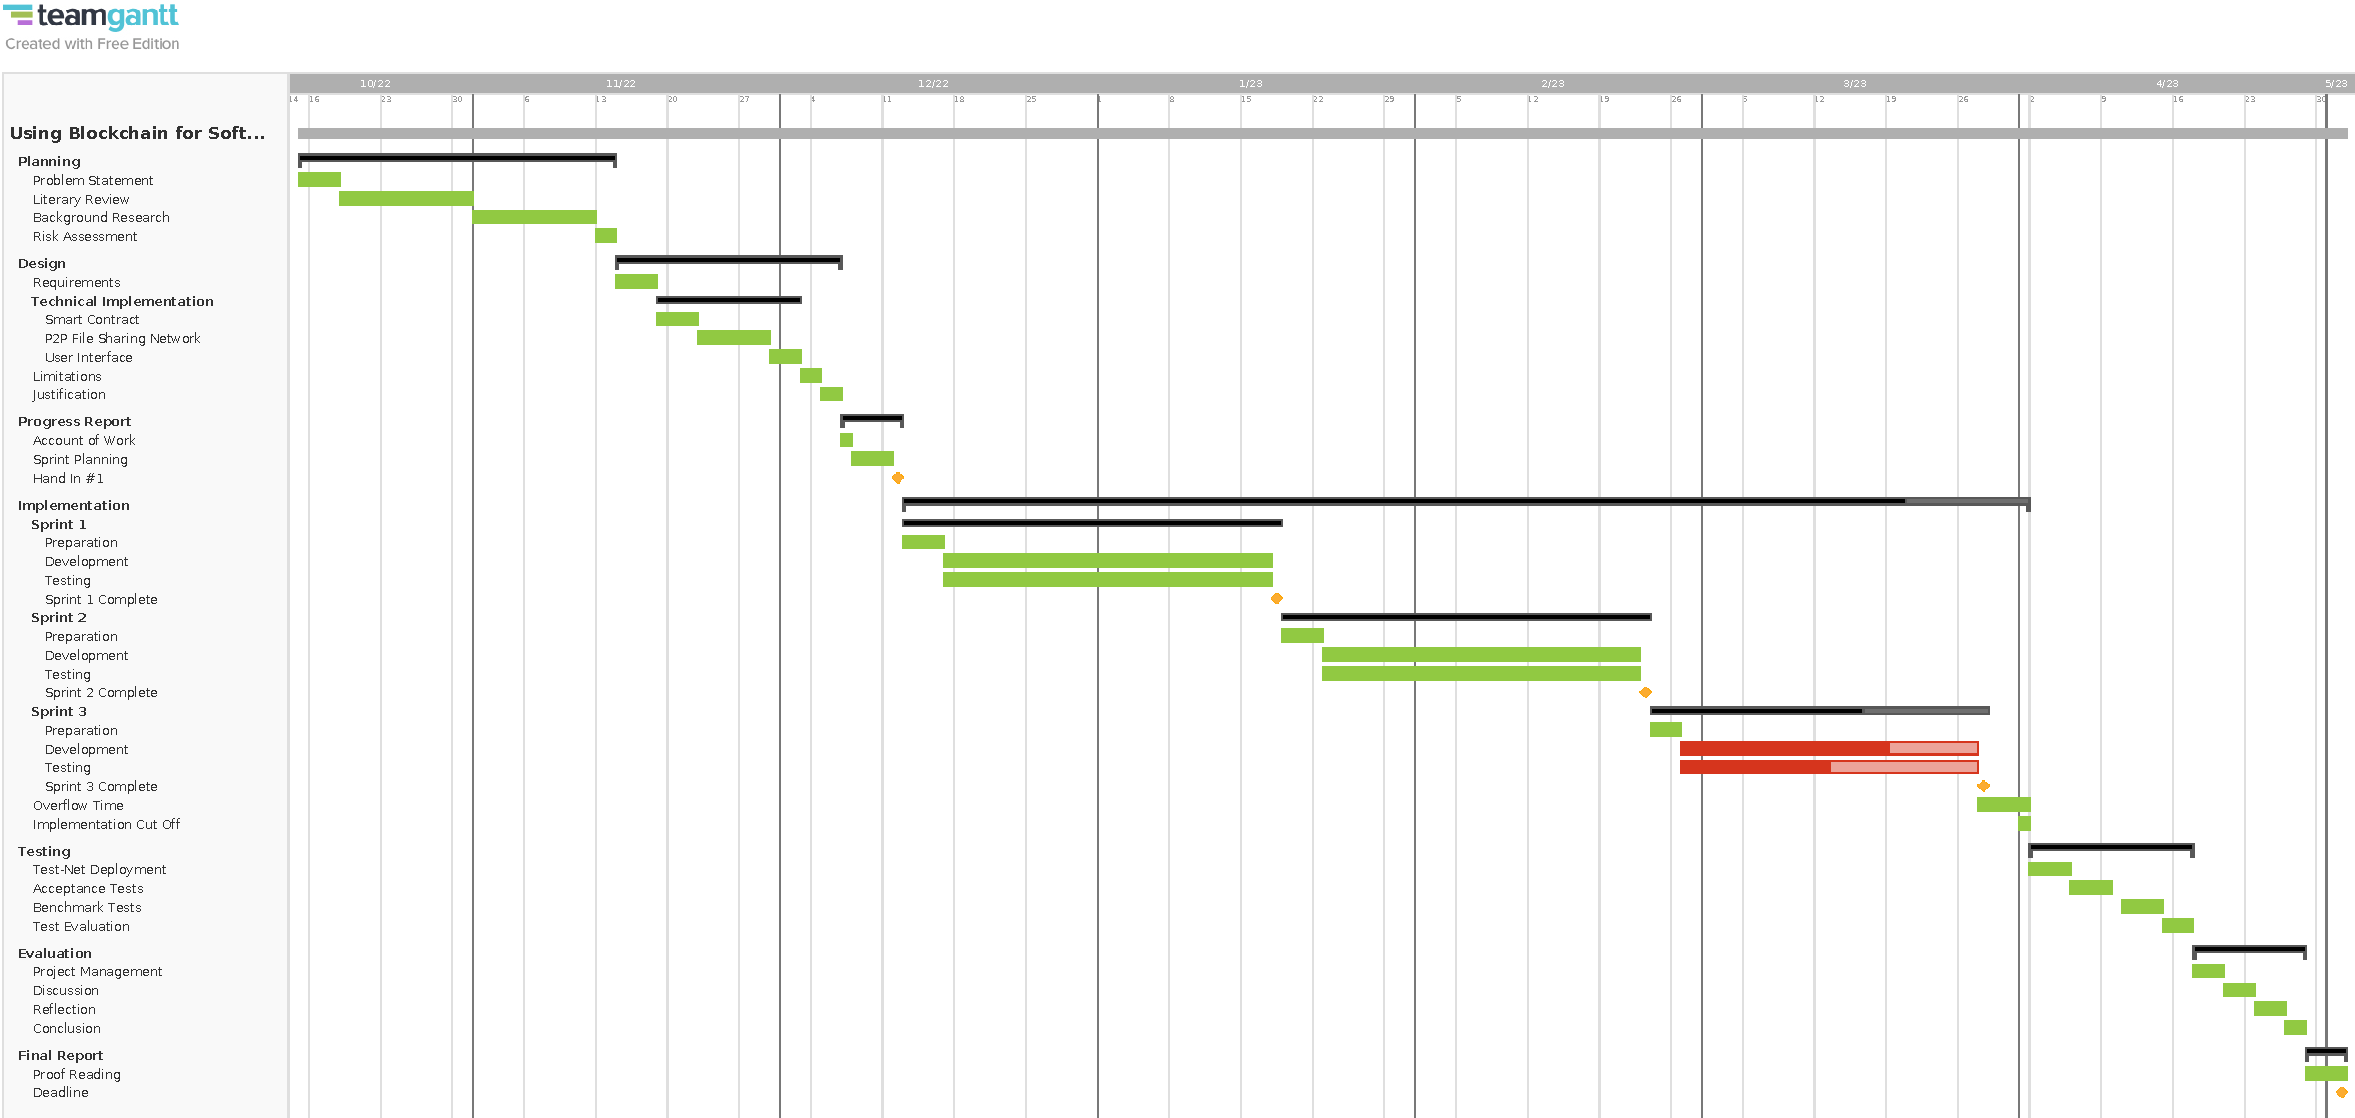
\includepdf[angle=90, scale=.95]{assets/gantt/gantt-a3-cropped.pdf}
    \vspace{150mm}
    \caption{The Gantt chart showing a breakdown of my project by task and milestones, where the red areas indicate incomplete work. Created with TeamGantt~\cite{noauthor_free_nodate}.}
    \label{fig:gantt-chart}
  \end{figure}
\end{landscape}
